\chapter{Knowledge to be gained from \textit{The Visual Display of Quantitative Information} facing CIRDLES' new ploting library.}

\section{Introduction}
Topsoil is the latest projet from the CIRDLES' lab. It allow geochronologists to plot various graphs needed for the analysis of aliquots. This software is based on the JavaFX library which gives to Java the ability to display user interfaces.

The first and current version of Topsoil is using the ploting abilities of JavaFX. But as we copied and rewrite part of these to make them fit our needs, we quickly realized that they had too much flaws to be a long term solution.
 Being a long term solution is one of Topsoil's objective. We needed another library to plot our graphic.

After a long and laborious search, John did not found one that could plot graphics for us. The solutions were either too specific, not well-designed enough or not compatible with JavaFX. From that moment on, it became clear that we needed to create our own graphic library. 

Although designing, coding and maintaining this kind of library is a lot of work, the result will be worth the effort. It is still preferable that the team document itself before starting a project of this scale. 
In that regard, I've red \textit{The Visual Display of Quantitive Information} by Edward Tufte and gathered some informations, presented in this rapport.
\\

This document is structured in three parts : 
\begin{itemize}
\item First of all, a very brief summary of the book will be given, allowing the reader to feel its tone.
\item Then charts that the library should be able to produce and their interesting particularities will be shown.
\item Finally, some of Tufte's rules for making good diagrams that the library should enforce or encourage to enforce will be listed. 
\end{itemize}
\emph{Please note that the recommendations contained in that report should not be exactly followed right away. They are useful to see the big picture.}%To be rephrased




\section{A quick summary of this book}
This book is a manifesto. It assert that charts are powerful tools of communication, explain why and how to make great graphics.
Along the book, Tufte find regrettable the underusage of plots in many kinds of publications, like textbooks, papers or journals. He also list a few reason of this underusage.

In the first part of his book, great graphs are listed. Then, errors that cause the integrity of the graph are given. Tufte describe the separation of graph and text, and the unfortunate simplicity of most of today's chart.
Finally, a set of rules that make great diagrams are given.




\section{A list of graphic}
It has been decided that our library should support a lot of type of graphics. To expend the range of known type by the team and gather documentation in one place, a number of chart along with the features needed in order to support them will be given here.

\subsection{Data Map chart}
Laying out data on a map can with no doubt, can carry an enormous volume of data and have a lot of reading levels.

%Complexe line representing the sea.
\centerline{
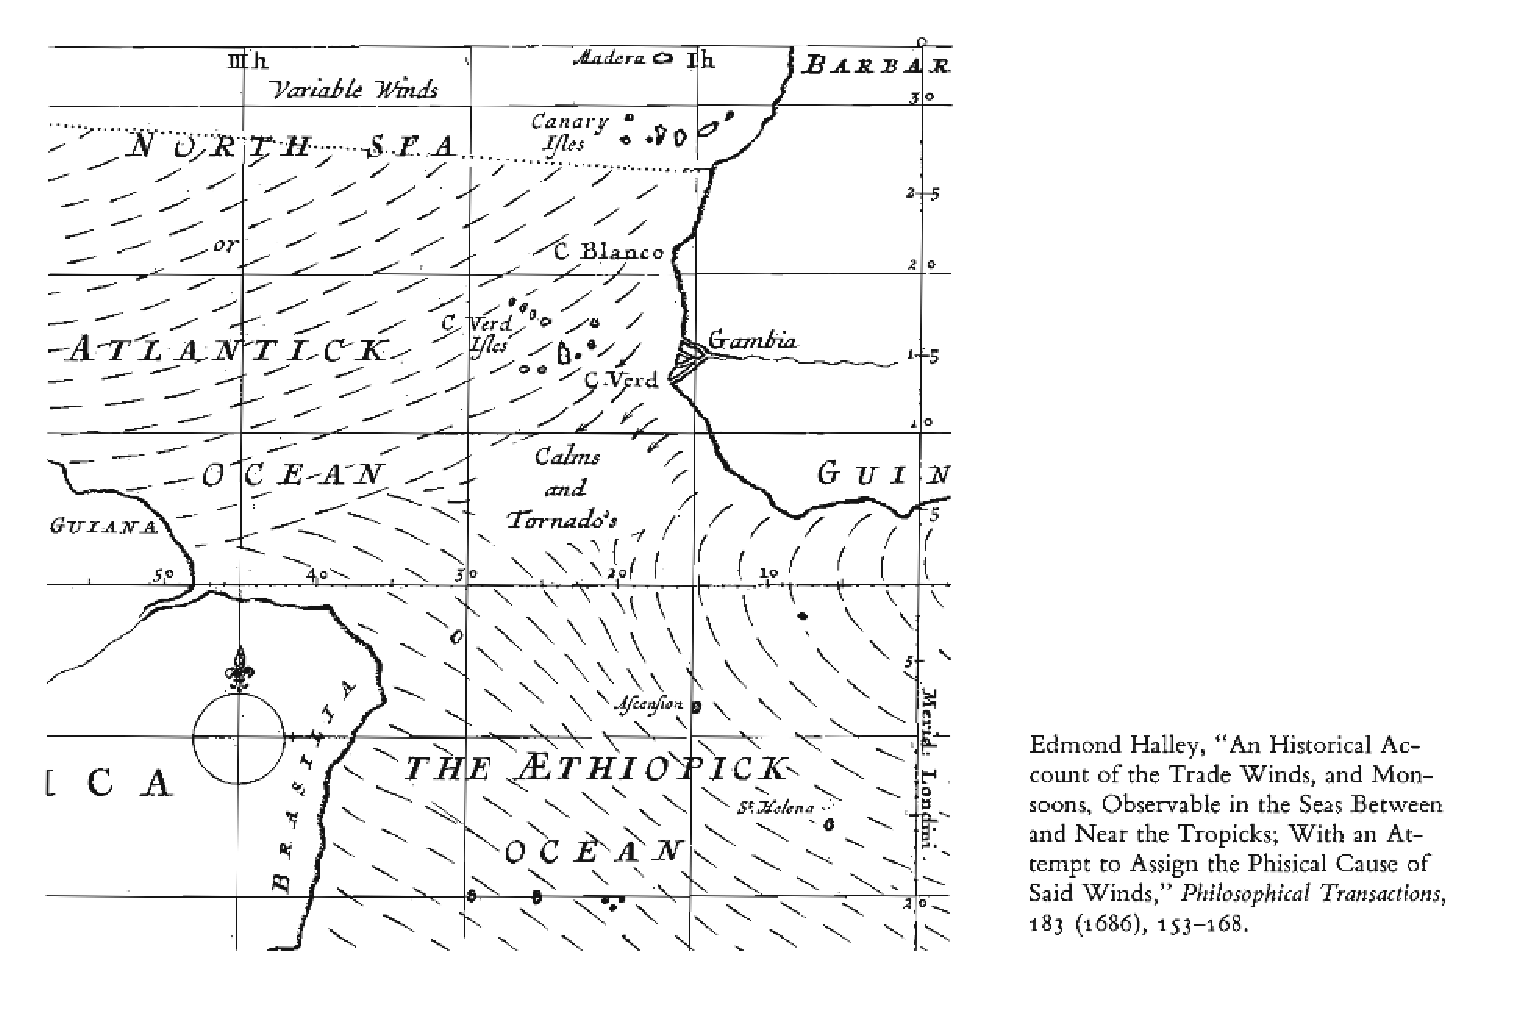
\includegraphics[width=19cm]{./illustrations/annexes/carte_courants.eps}
}
To implement this map, the \textit{Tufte} library's graph background would have to be be filled up with a map\footnote{It could be useful to look into interoperable map format, or even map libraries}, integrating name of landmarks. Symbols of all kind could be added, from a single point on a city to complex lines representing the sea like here :

%Cancer map
\centerline{
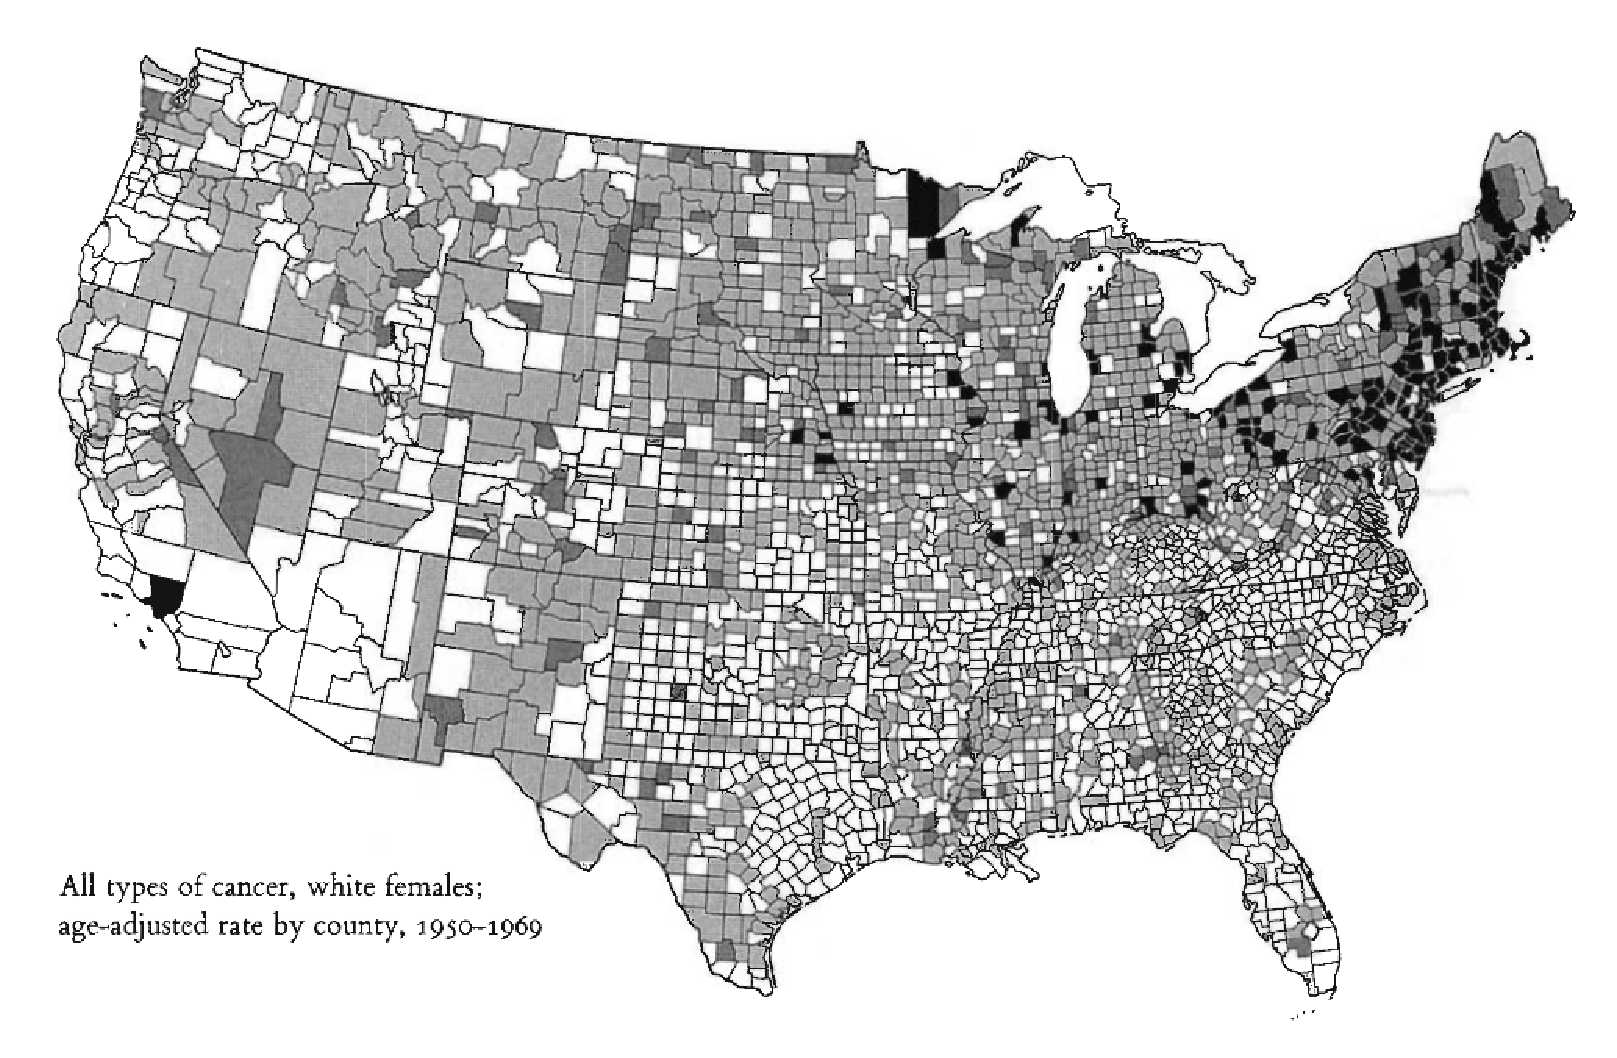
\includegraphics[width=19cm]{./illustrations/annexes/carte_cancer.eps}
}
An other important feature to consider for the library to implement this map is the binding of data to zone on the map in the background.

%French export
\centerline{
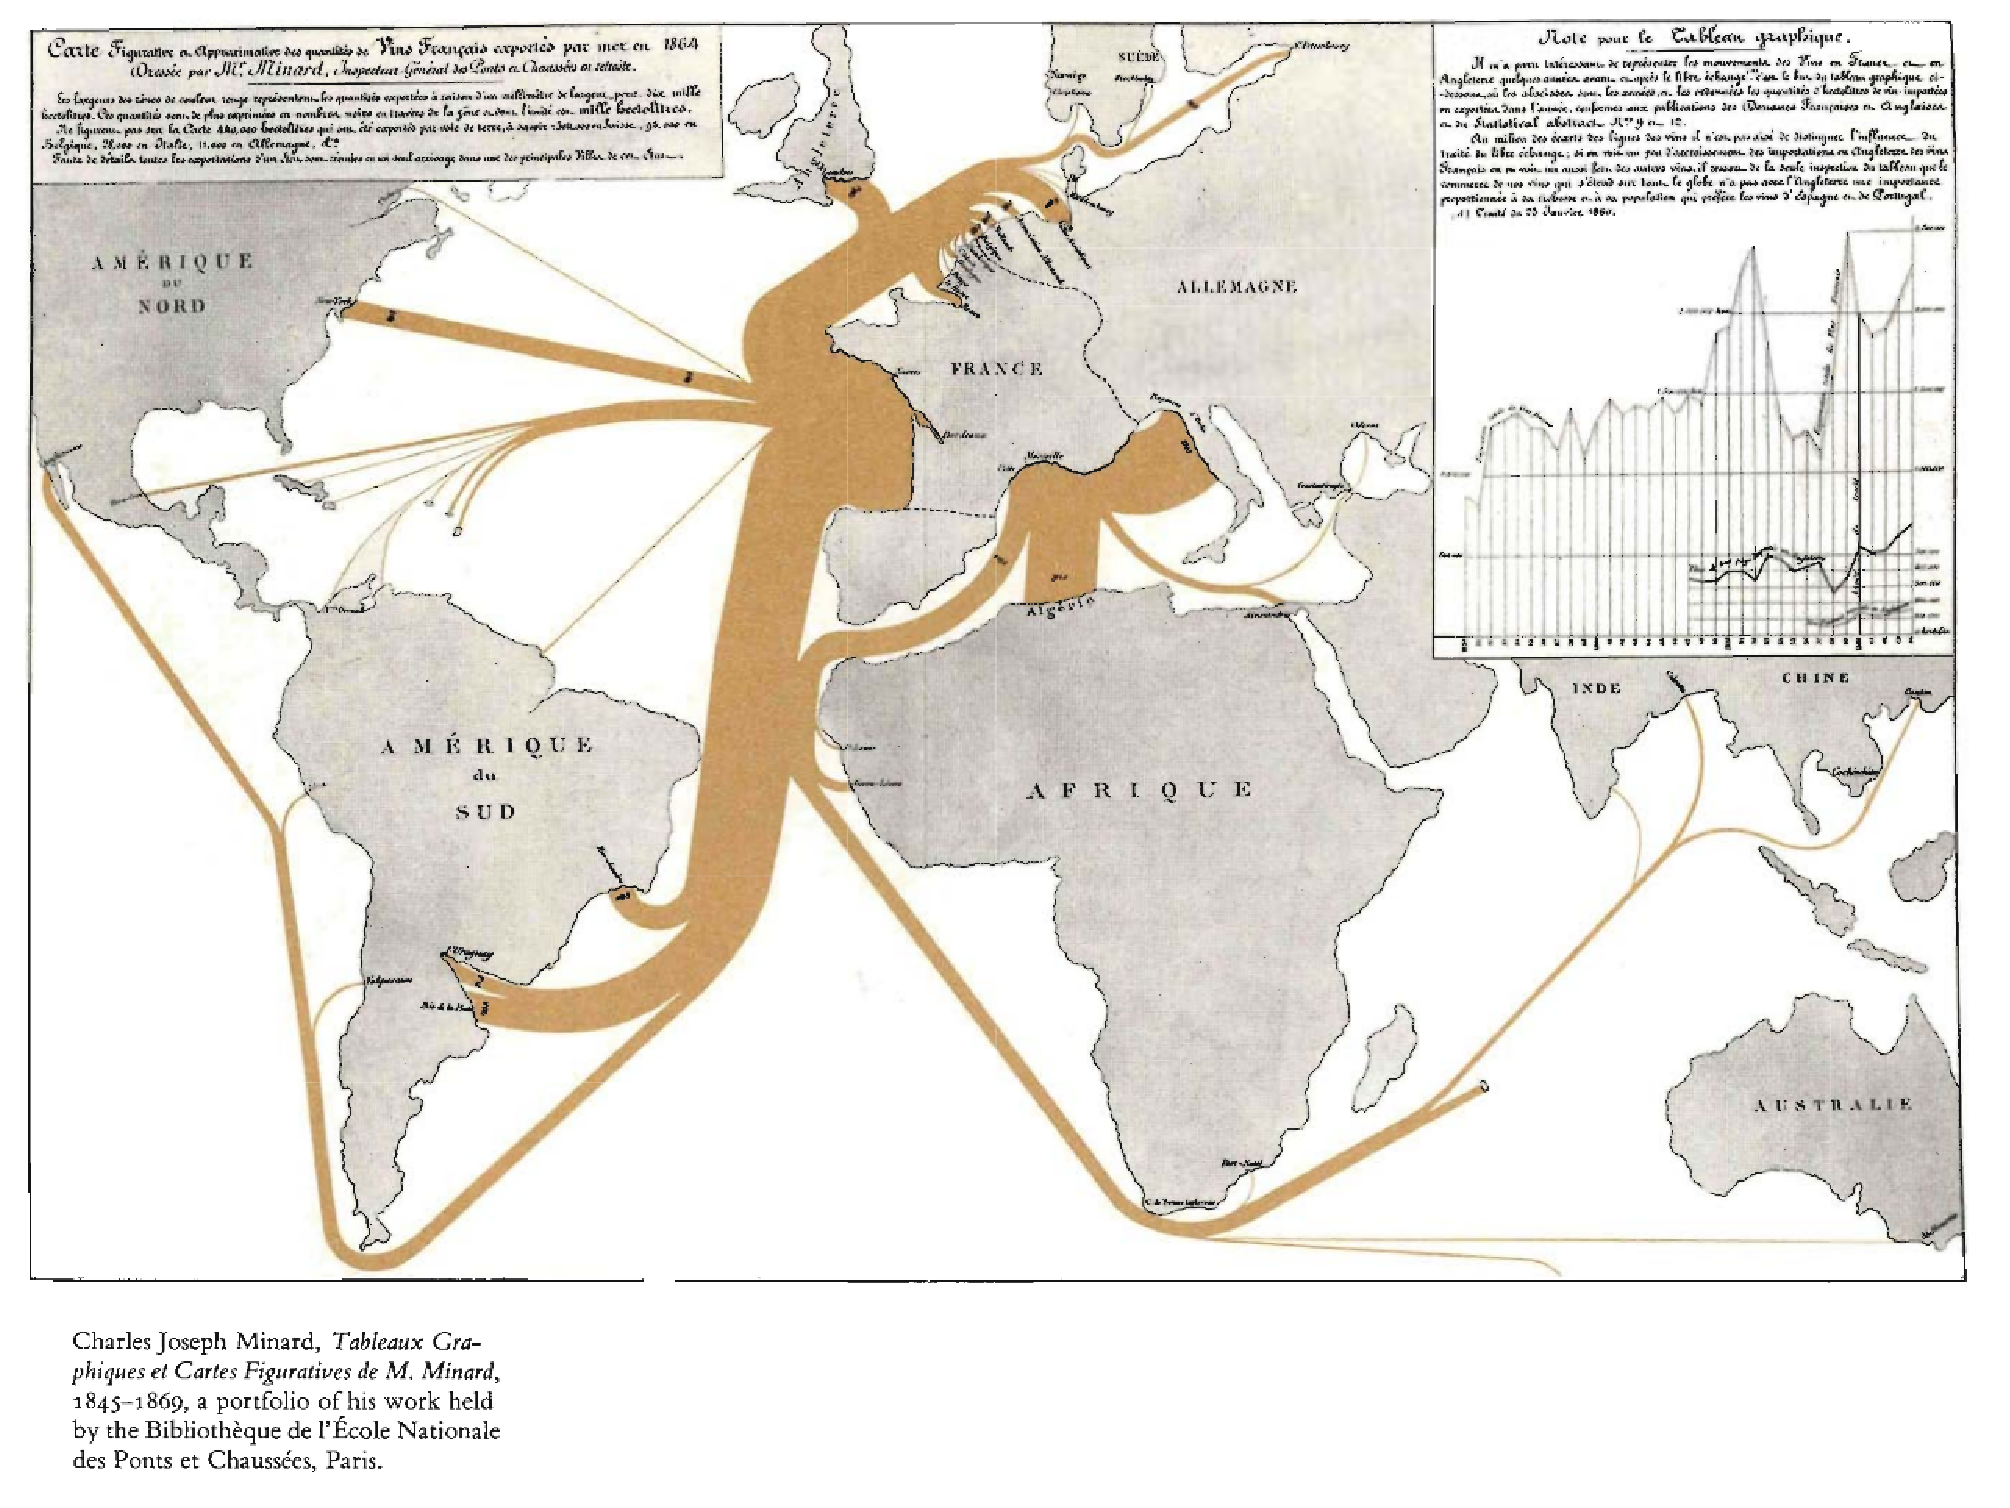
\includegraphics[width=19cm]{./illustrations/annexes/carte_exports.eps}
}
To draw this map, several layers of the map have to be known by the rendered line. The informations passed to draw theses are :
\begin{itemize}
\item Position of the begining
\item Position of the end
\item A quantity
\end{itemize}
The quantity is then turned into the width of line, which will be drawn from its begining to its end, without crossing earth.
The begining and the end must also fit closely the earth. These are the two reasons why the rendered elements should be awared of the map and its shape.

\subsection{Time-Space chart}
%NY City Weather
\centerline{
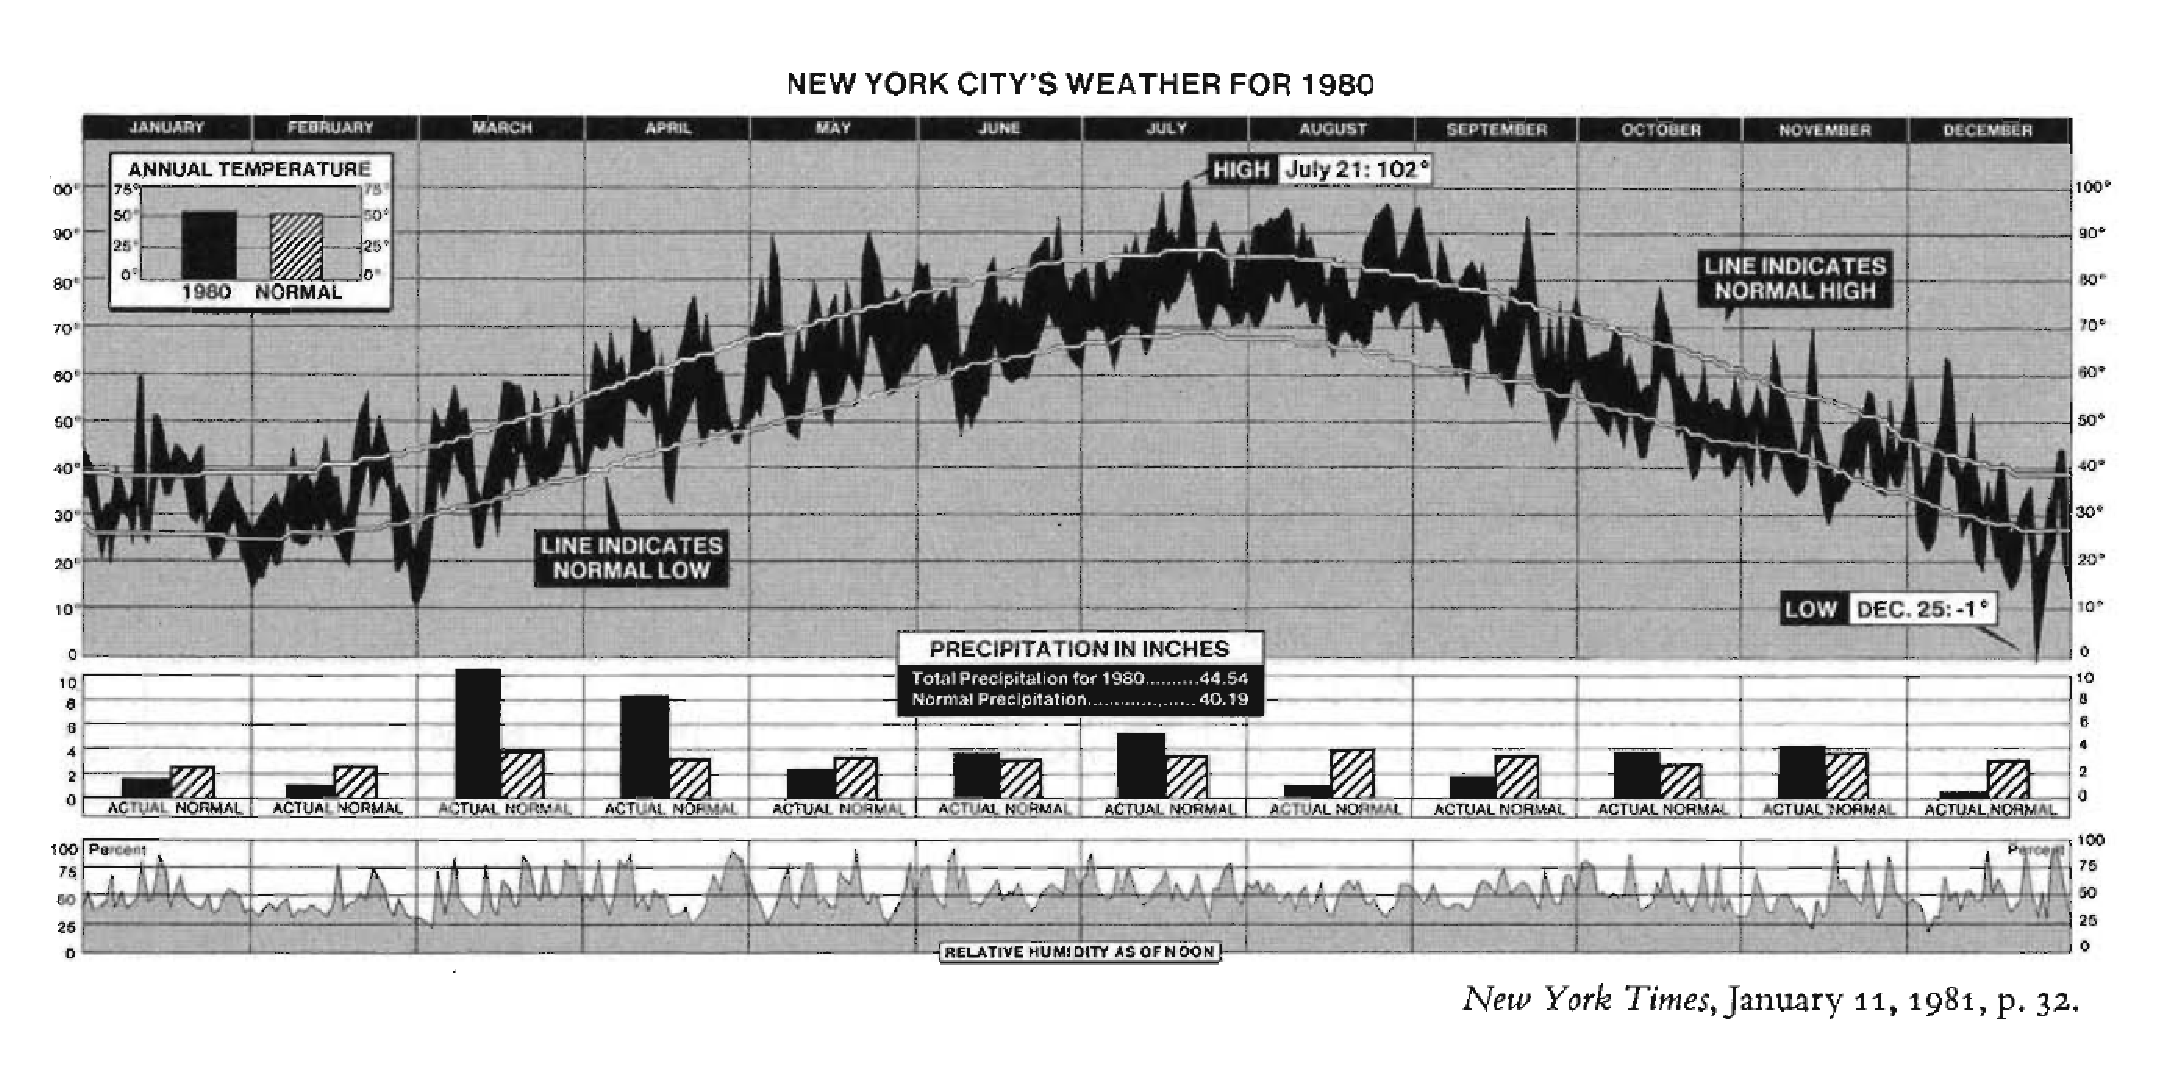
\includegraphics[width=19cm]{./illustrations/annexes/temps_nymeteo.eps}
}
Several informations can be gained from that plot.

First, notice the indications pointing on the main curve (like "LINE INDICATE THE NORMAL LOW"). Tufte love their usefulness. We should find a way to make them point to either a point of a serie of point, or to nothing. Also, allow the automation to print the data they are pointed to
Secondly, notice that the temperature axis is reproduced on the two sides. Printing the same axis mutliple time on the same plot should be a possibility. 
Thirdly, there is one subgraph drawn for each month representing the difference between the actual precipitation and the normal.
Last, but not least : the several pieces of data are linked to the same x-axis and to different y-axis.

%Playfair : "Sharing at one wiew the Price of Quarter of Wheat ...
\centerline{
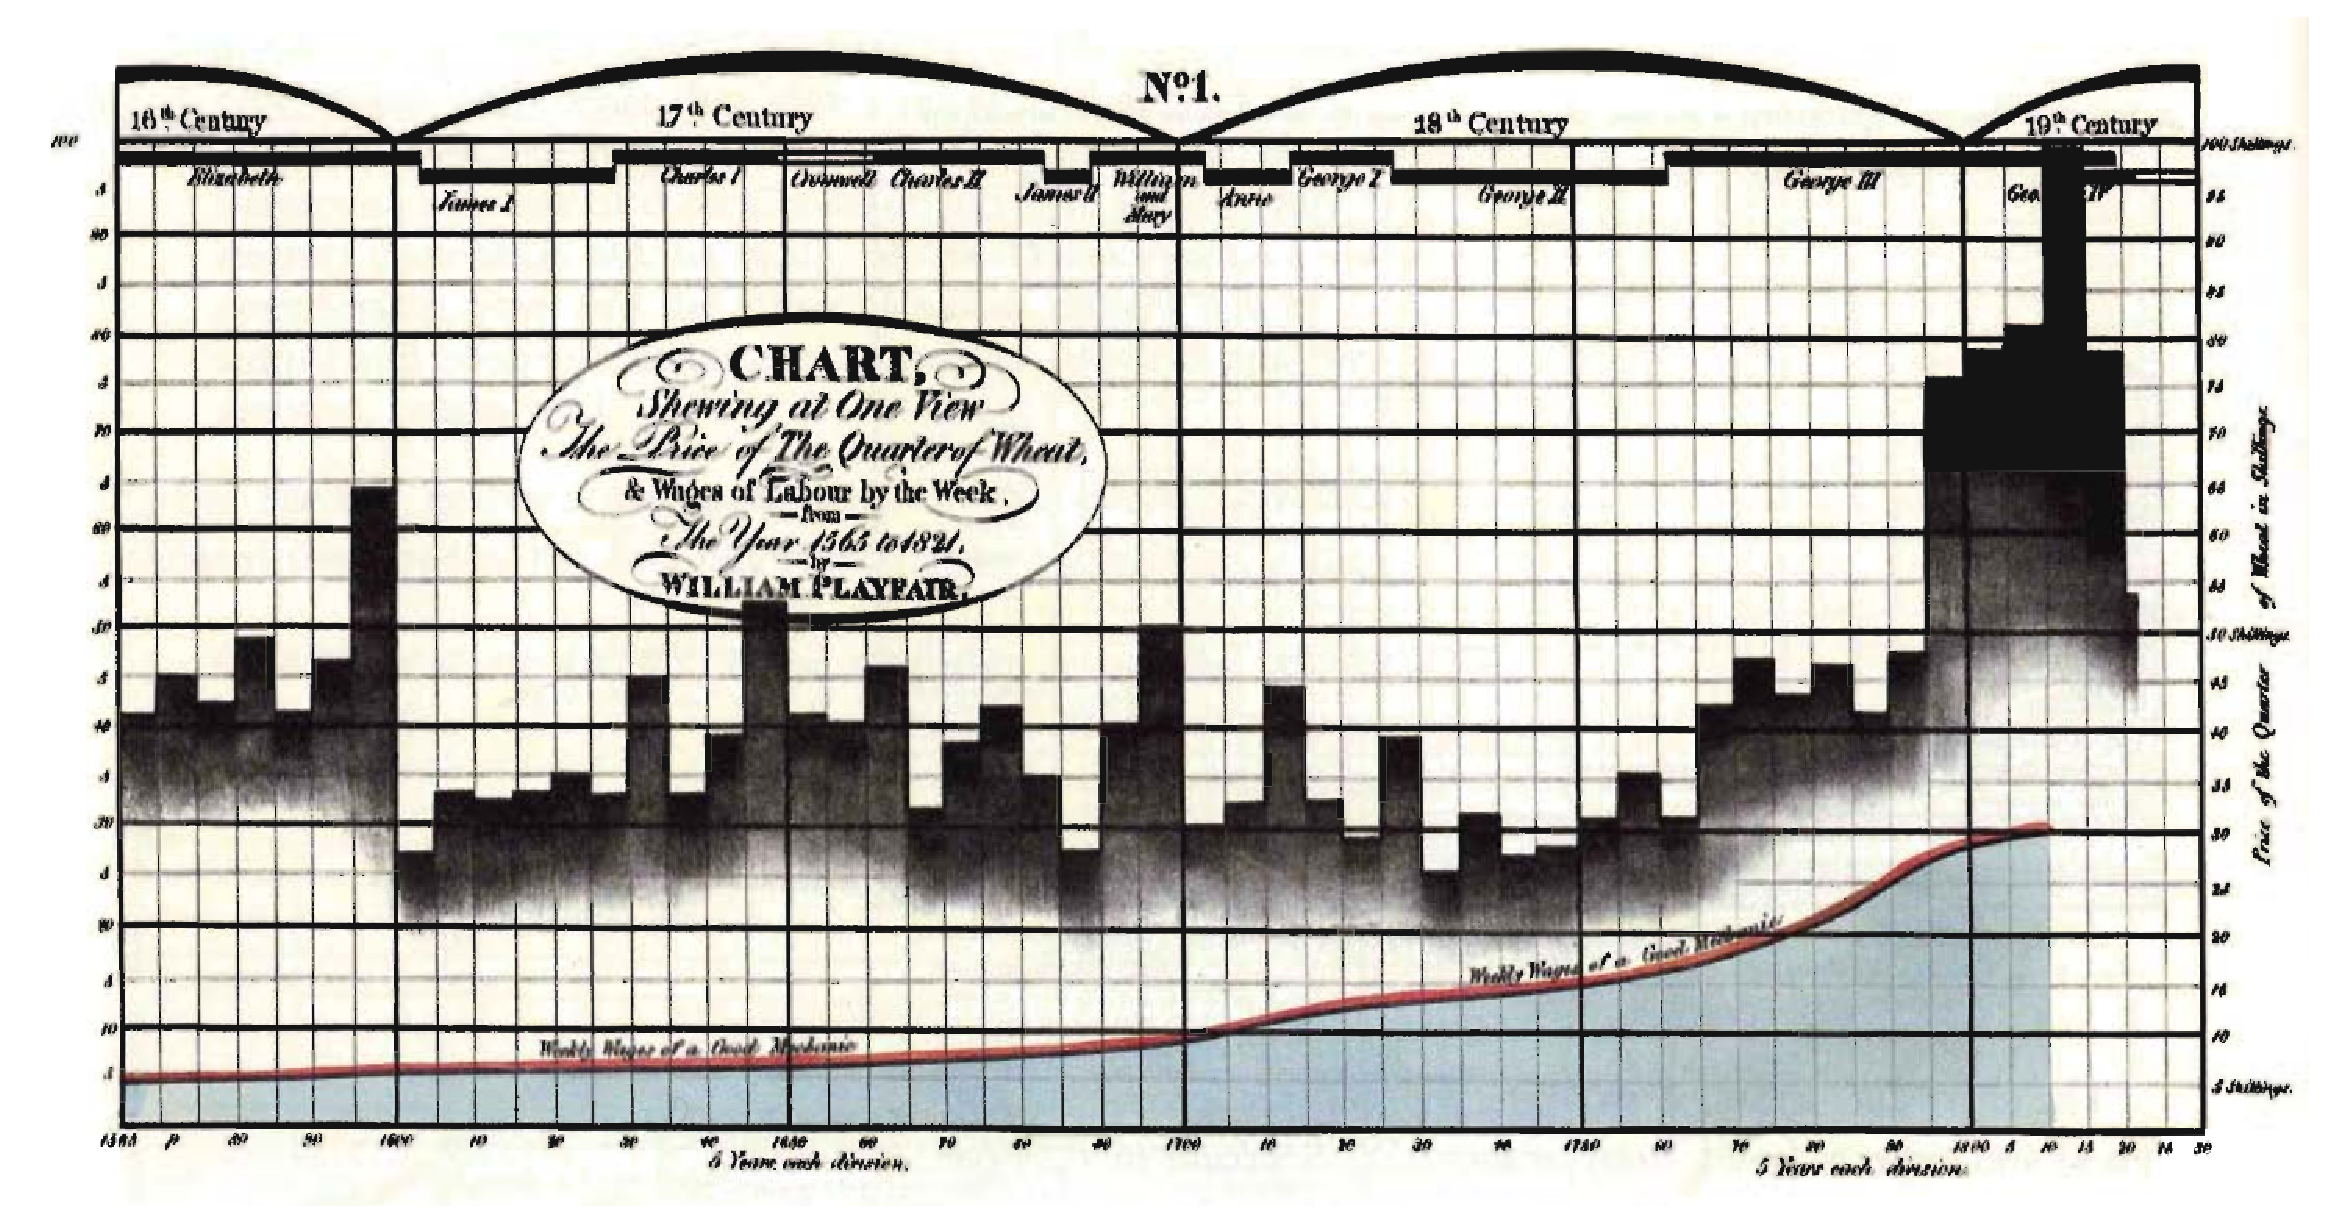
\includegraphics[width=19cm]{./illustrations/annexes/temps_ble.eps}
}
Concernine this diagram, I cannot think of more than one axis of reflection for now. There are two sets of data that have there own space, making the plot more readable. Maybe we could arrange plot of data to be aware of their sibblings, or make the PlotArea smarter when it is outlining two set of data.

%http://worldtracker.org/media/library/Science/Science%20Magazine/science%20magazine%201981-1982/Science%201981-1982/root/data/Science_1981-1982/pdf/1982_v216_n4550/p4550_1086.pdf

\subsection{Time-Space chart}
%Teh Napoleon Chart
\centerline{
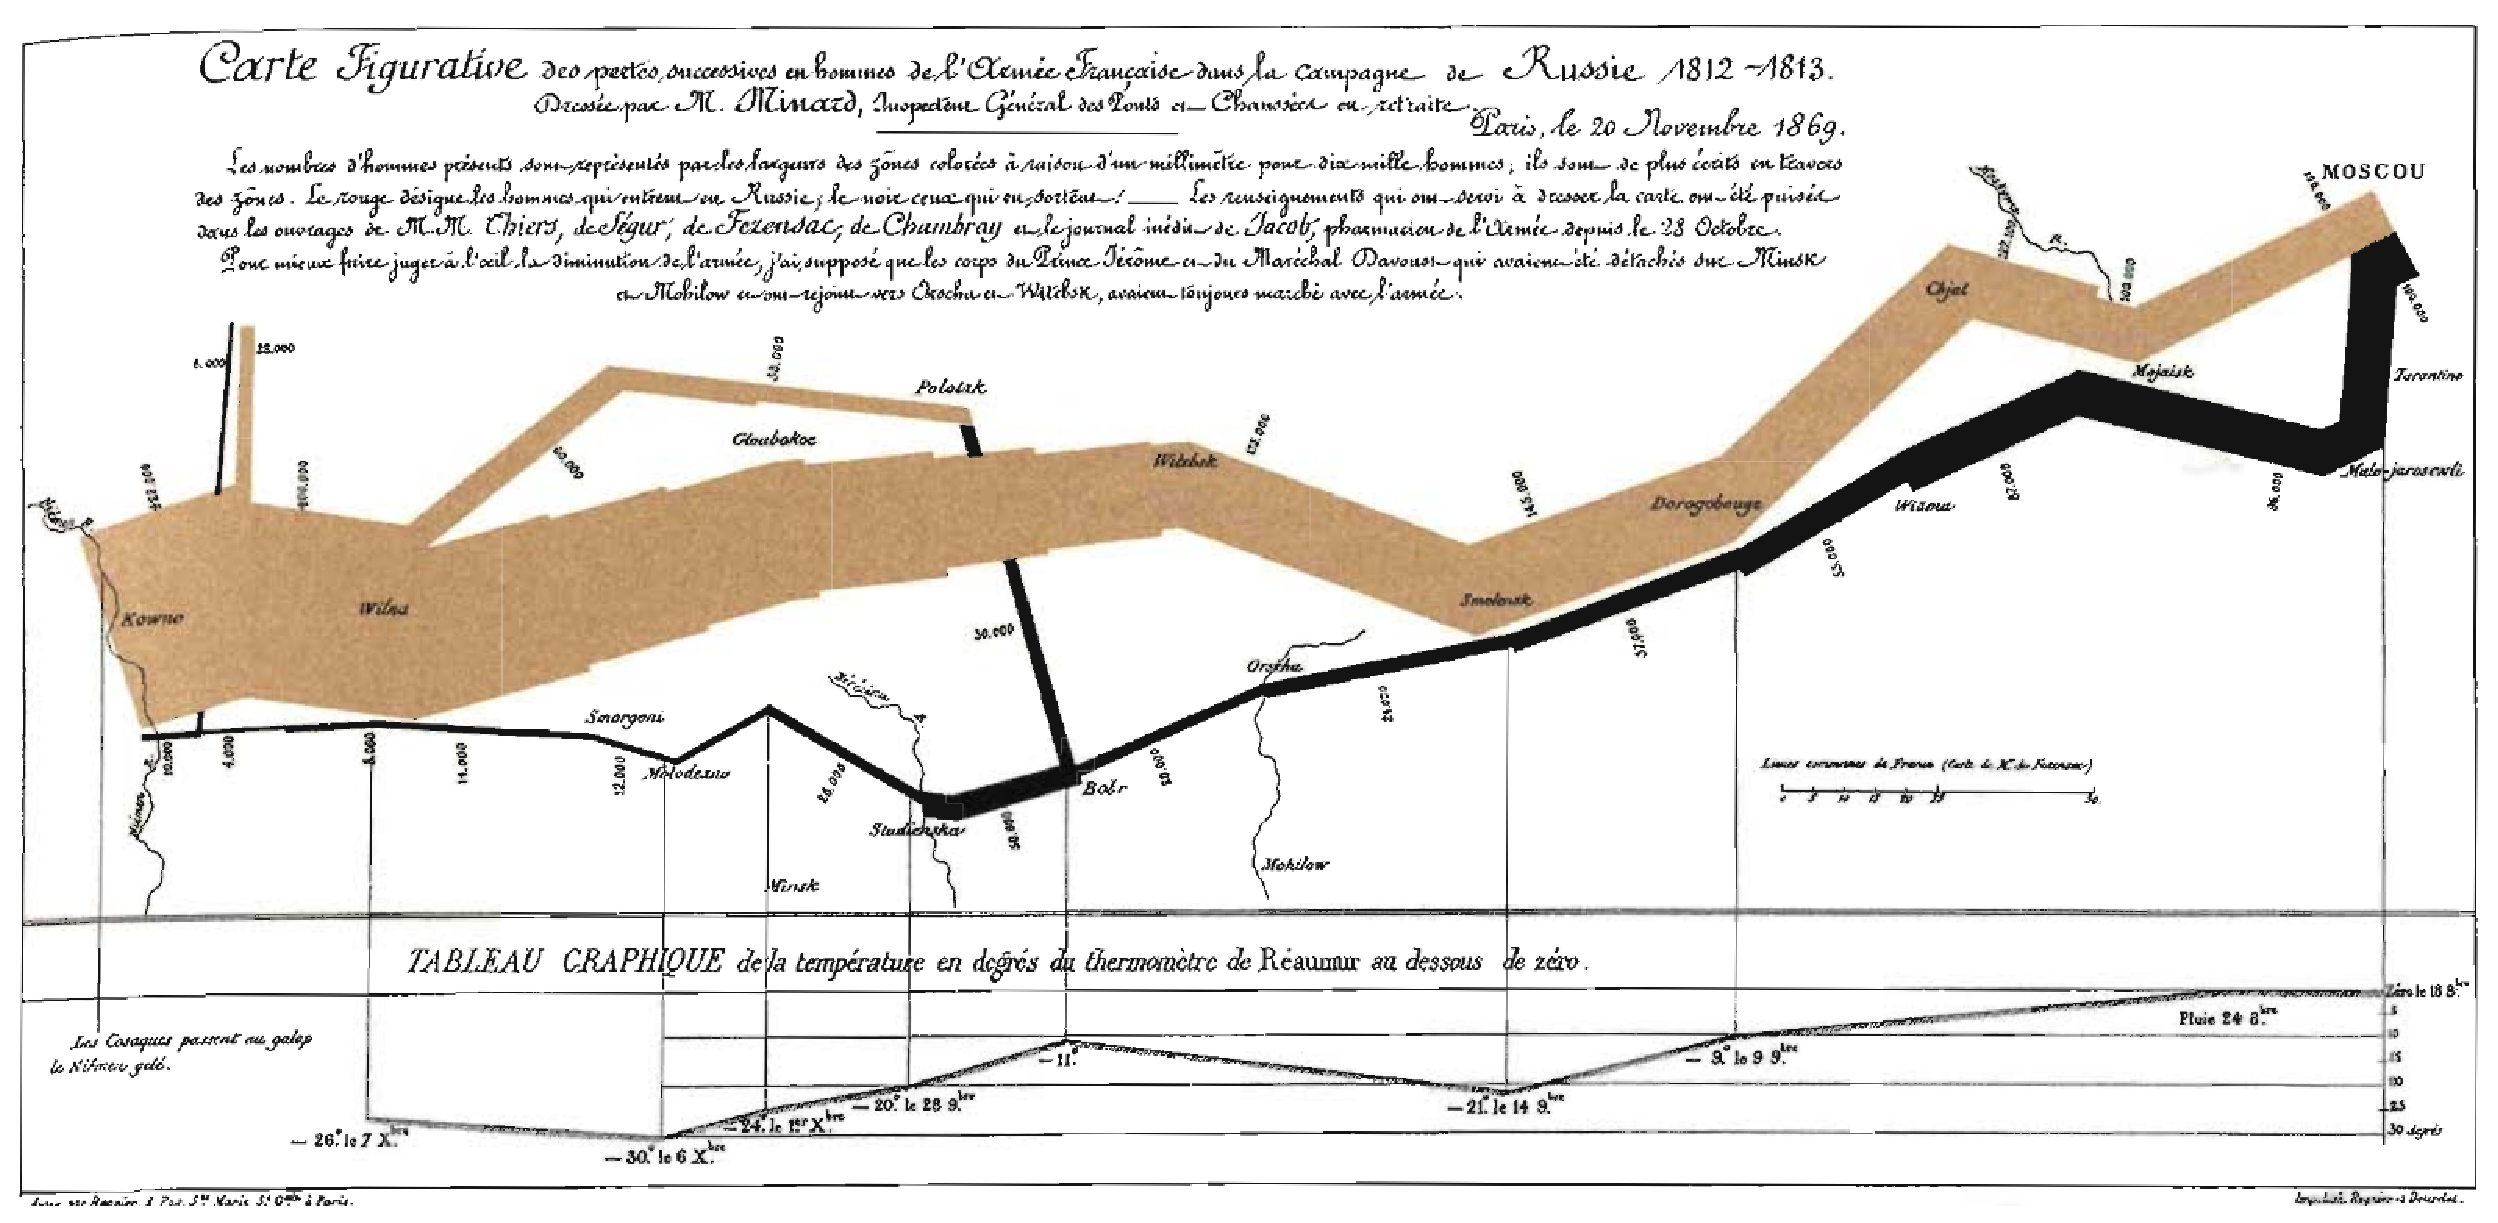
\includegraphics[width=19cm]{./illustrations/annexes/tempscarte_napoleon.eps}
}
The very interesting construction of the diagram is here made in two times. The following data is given to draw the path of Napoleon's army in russia, for each step : the two numbers of the location of the step, the number of soldier (transformed in the width) that was at that moment in the army, and the date which give the order\footnote{There is also the travel direction of the army that give the color, but it is not relevant in this context}.

There are two things to say about that. The plot of a serie of data can not be made of several plot of the different point that it is made of : there is also information about the link between all those plot. For exemple, here, if we ploted all the plot one at the time, the location would be drawn, but not the path between two of those location.
Let's now take a look at the bottom of the chart, where the temperature of each steps is represented. The x-axis is simply representing the temperatures. The y-axis on the other hand is "the step", and is given by the first and main plot of the diagram. This is a very interesting use case.

\section{Several principles that make a good plot}
Edward Tufte give in his book several principles that make a good chart. For the moment, I do not certify that all of those rules will be of some help for our work. I still think the team should be aware of their existence.

There are two sort of rules :
\begin{itemize}
\item Those which avoid misleading diagram  
\item Those which allow a better presentation of the plot
\end{itemize}

\subsection{Keeping graphical integrity} 
Tufte put together five rules that must be followed when building a graph to ensure its integrity.

\begin{quote}
The representation of numbers, as physically measured on the surface of the graphic itself, should be directly proportional to the numerical quantities represented.
\end{quote}
This is not always the case and lead to misinformation of the uncareful viewer. Tufte invented a unit representing how much the diagram is lying : the Lie Factor.

$Lie Factor = \frac{size of effect shown in graphic}{size of effect in data}$

A quick exemple of the Lie Factor :

%Image of the Fuel Economy Standards for auto
\centerline{
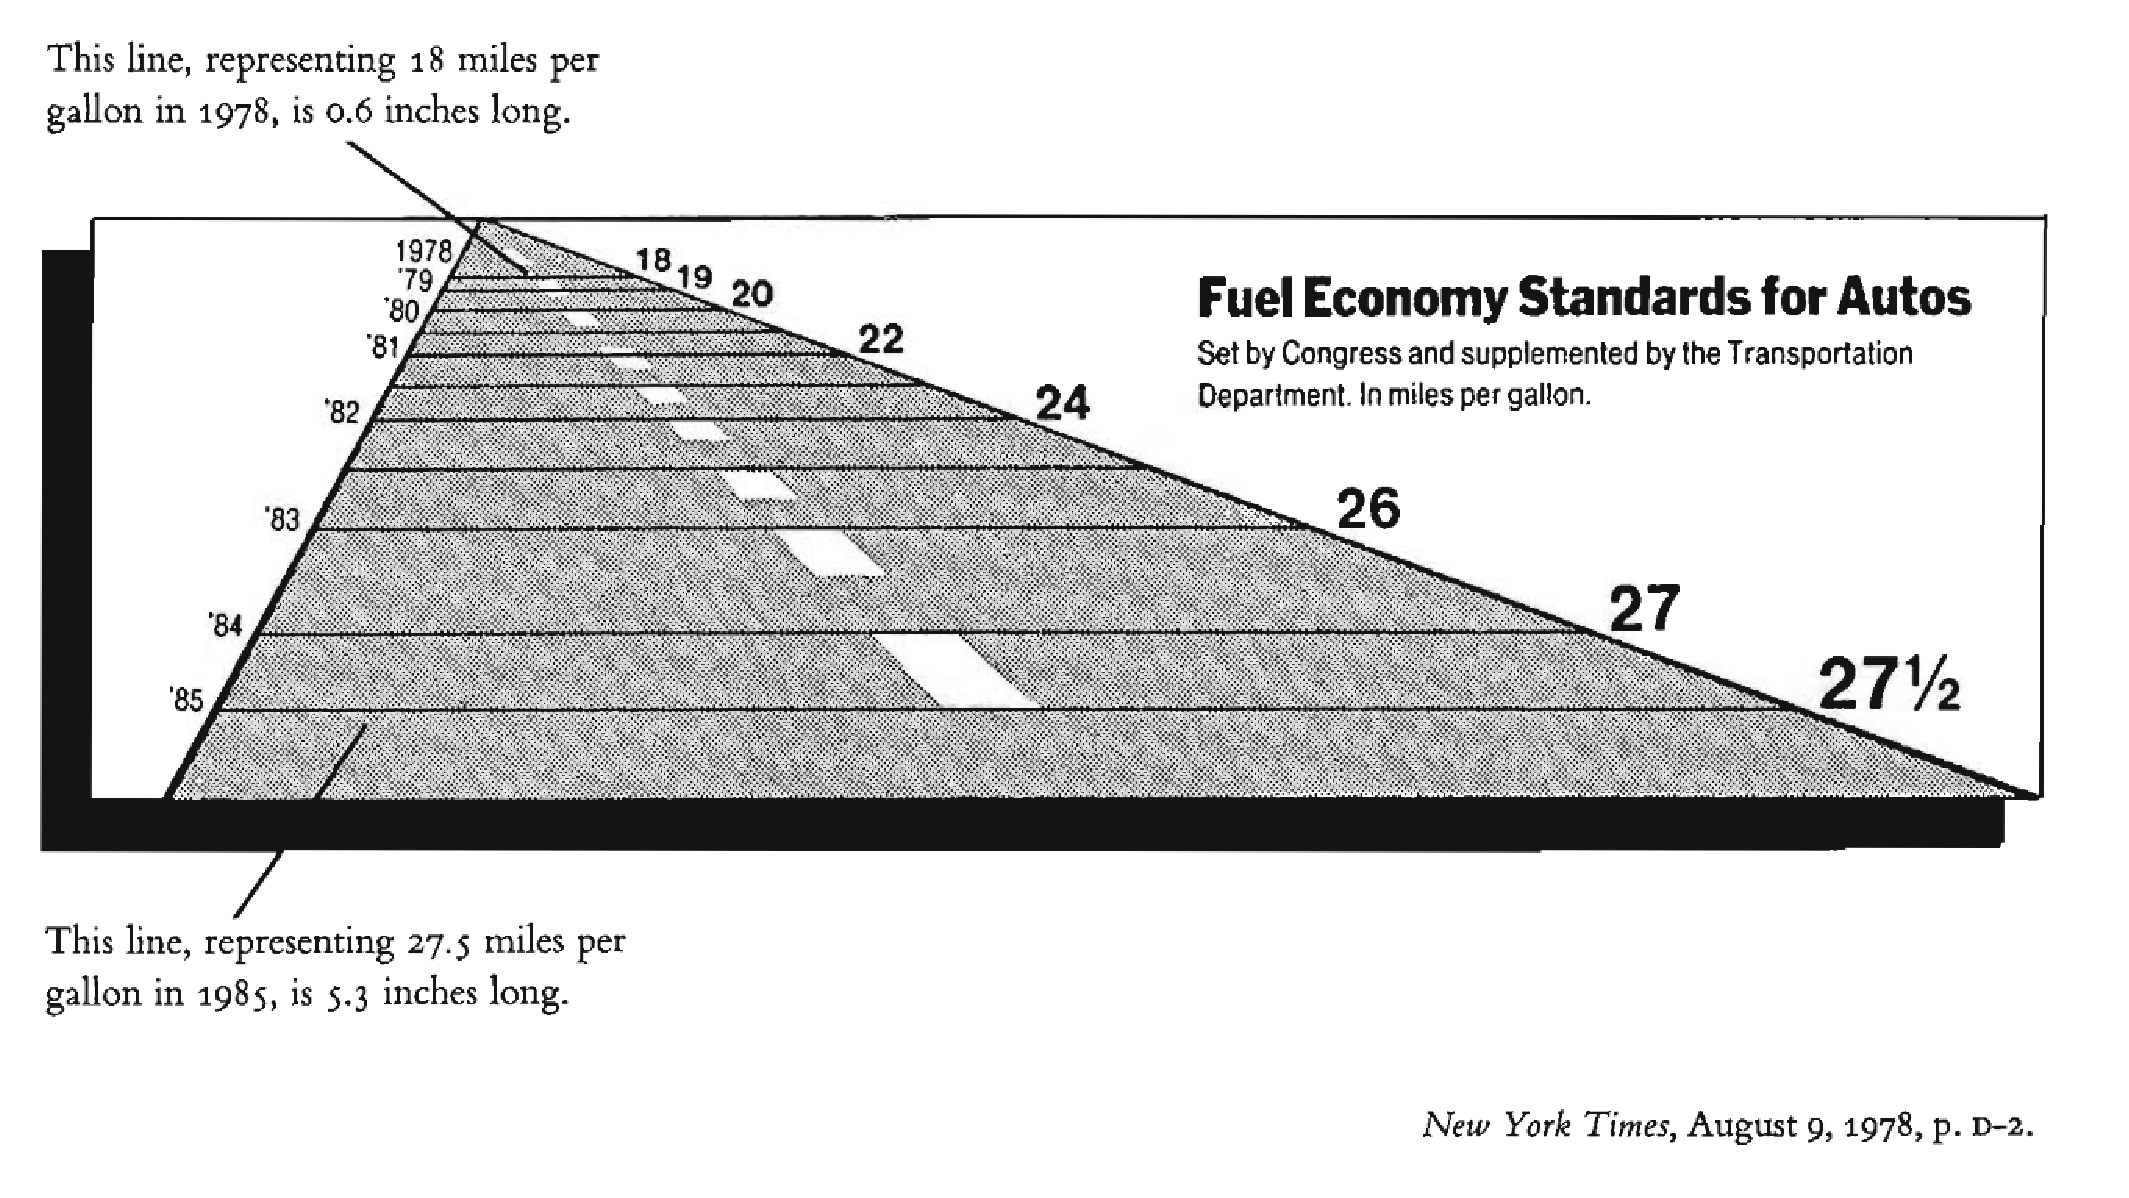
\includegraphics[width=19cm]{./illustrations/annexes/temps_fuel.eps}
}

\begin{itemize}
\item The increase between 18 and 27 is \emph{53\%}
\item The increase between 0.6 inch and 5.3 inch, the size of the two side of the road is \emph{783\%}
\end{itemize}

The lie factor is  : $\frac{783}{53} = 14.8$ 

\begin{quote}
Clear detailed and thorough labeling should be used to defeat distortion and ambiguity. Write out explanations of the data on the graphic itself
\end{quote}

As said before, the library should provide a way to add text, possibly linked to the data, or the serie of data.
\begin{quote}
Show data variation, not design variation.
\end{quote}
The unit on the axis should never change. On some of the book's graphic, on the x-axis, the section between represent a year.
Then, for the same lengh, it suddenly switch to one month. It is not may obvious and the unfocused viewer suddenly see a drop in the data. 
Also the aspect ratio of the graphic matters. A graphic taller than wide can depict a normal situation as skyrocketing.

\begin{quote}
In time-series displays of money, deflated and standardized units of monetary measurement are nearly always better than nominal unit
\end{quote}

\begin{quote}
The number of information-carrying (variable) dimensions depicted should not exceed the number of dimensions in the data.
\end{quote}
There are considerable ambiguities in how peoples percieve a two-dimensional surface, and making the area proportional to the data is a perilous task. For a single data, a single dimension form, like a line, is better.

\begin{quote}
Graphic must not quote data out of their context
\end{quote}

%Image of the nazi thingy
\centerline{
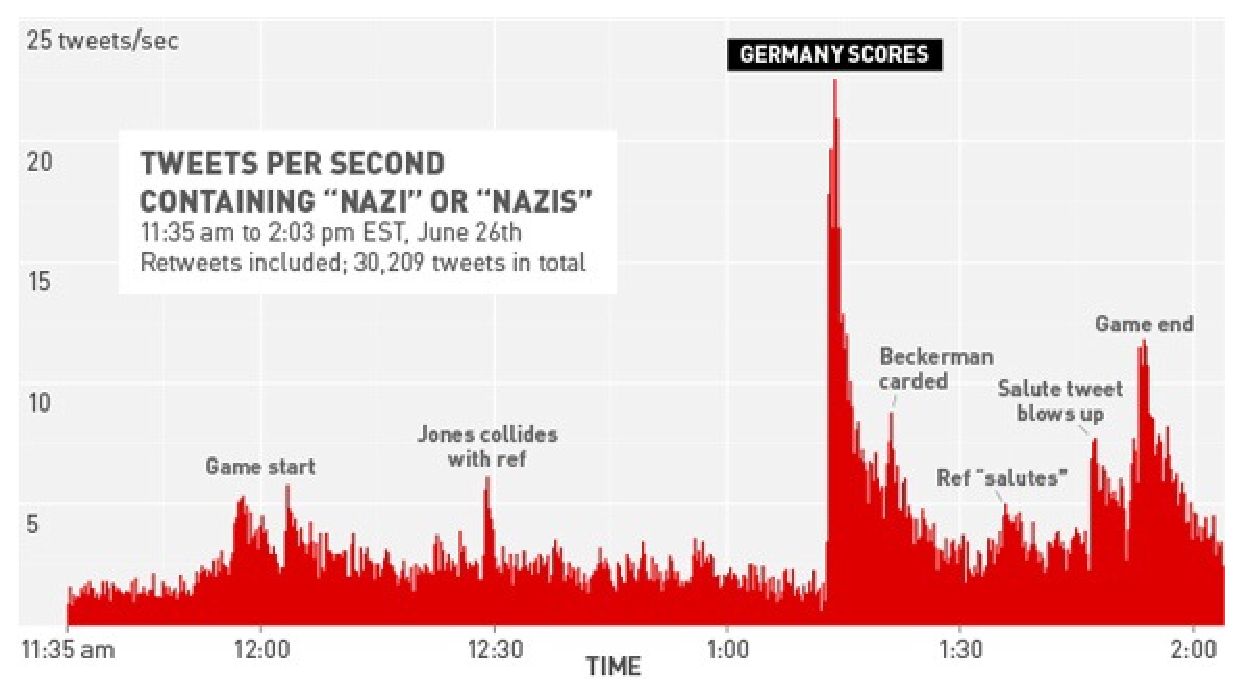
\includegraphics[width=19cm]{./illustrations/annexes/temps_nazi.eps}
}
This image shows us that the number of time by seconds the words "nazi" and "nazies" were tweeted during an USA vs. Germany match skyrocketed from 5 to 25 when Germany scored.
But none of the data shows us how many time the word is tweeted during the rest of the year. This is a problem because it could be a lot more than that or a lot less, and we have no ideas.

\subsection{Building clearer graphic}
\begin{quote}
Above all else, show the data
\end{quote}

Tufte believe that most of the ink/pixels of the chart should be used to draw the data. He even invented another ratio to measure how much the graphic was clogued up by unuseful drawings.

$Data-ink ratio = \frac{data-ink}{total ink used to print the graphic}$

The data ink comprise nothing exept the object representing the data. This means that the objects allowing the representation to make sense (axis, texts) are not included. 
This is why the data-ink ratio must most of the time never be one, but should stay near one.
A grid too precise, axis overloaded, unrelated drawing : all of those block a graphic, preventing it to deliver correctly the data.

%Image d'un histogramme
\centerline{
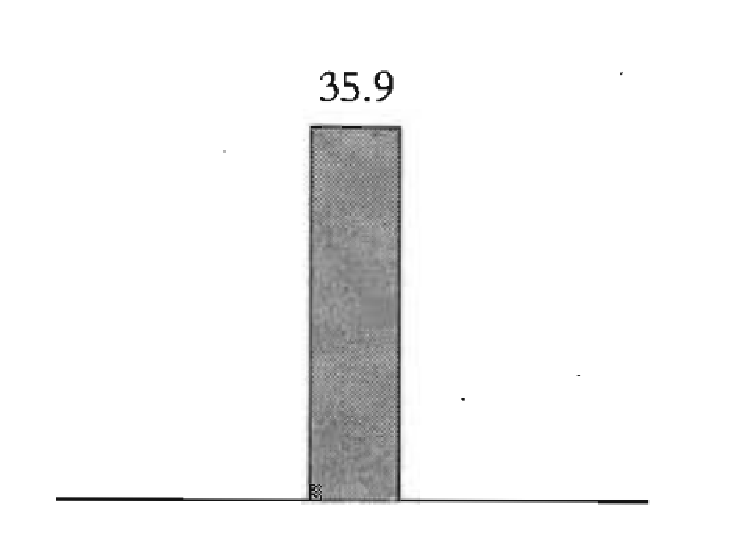
\includegraphics[width=19cm]{./illustrations/annexes/histogramme.eps}
}

Representing the data multiple time is also orverloading a chart. On this bar, the number "35.9" is represented in 6 ways :
\begin{itemize}
\item Height of the left line
\item Height of the right line
\item Height of the shading
\item Height of the top line
\item Position of the text
\item Text itself
\end{itemize}
This is ink lost and chart complexified for nothing. Remember, it's like in a movie : You don't need three shots of someone saying one sentence if one is as efficient. And you don't need to move around her unless you have a good reason 
 Damn you, Michael Bay.
 A chart creator should always try to represente one information with less ink as possible.
 One hint, in order to achieve this : Symmetry represent always represent the data twice.

%Image : Moire
\centerline{
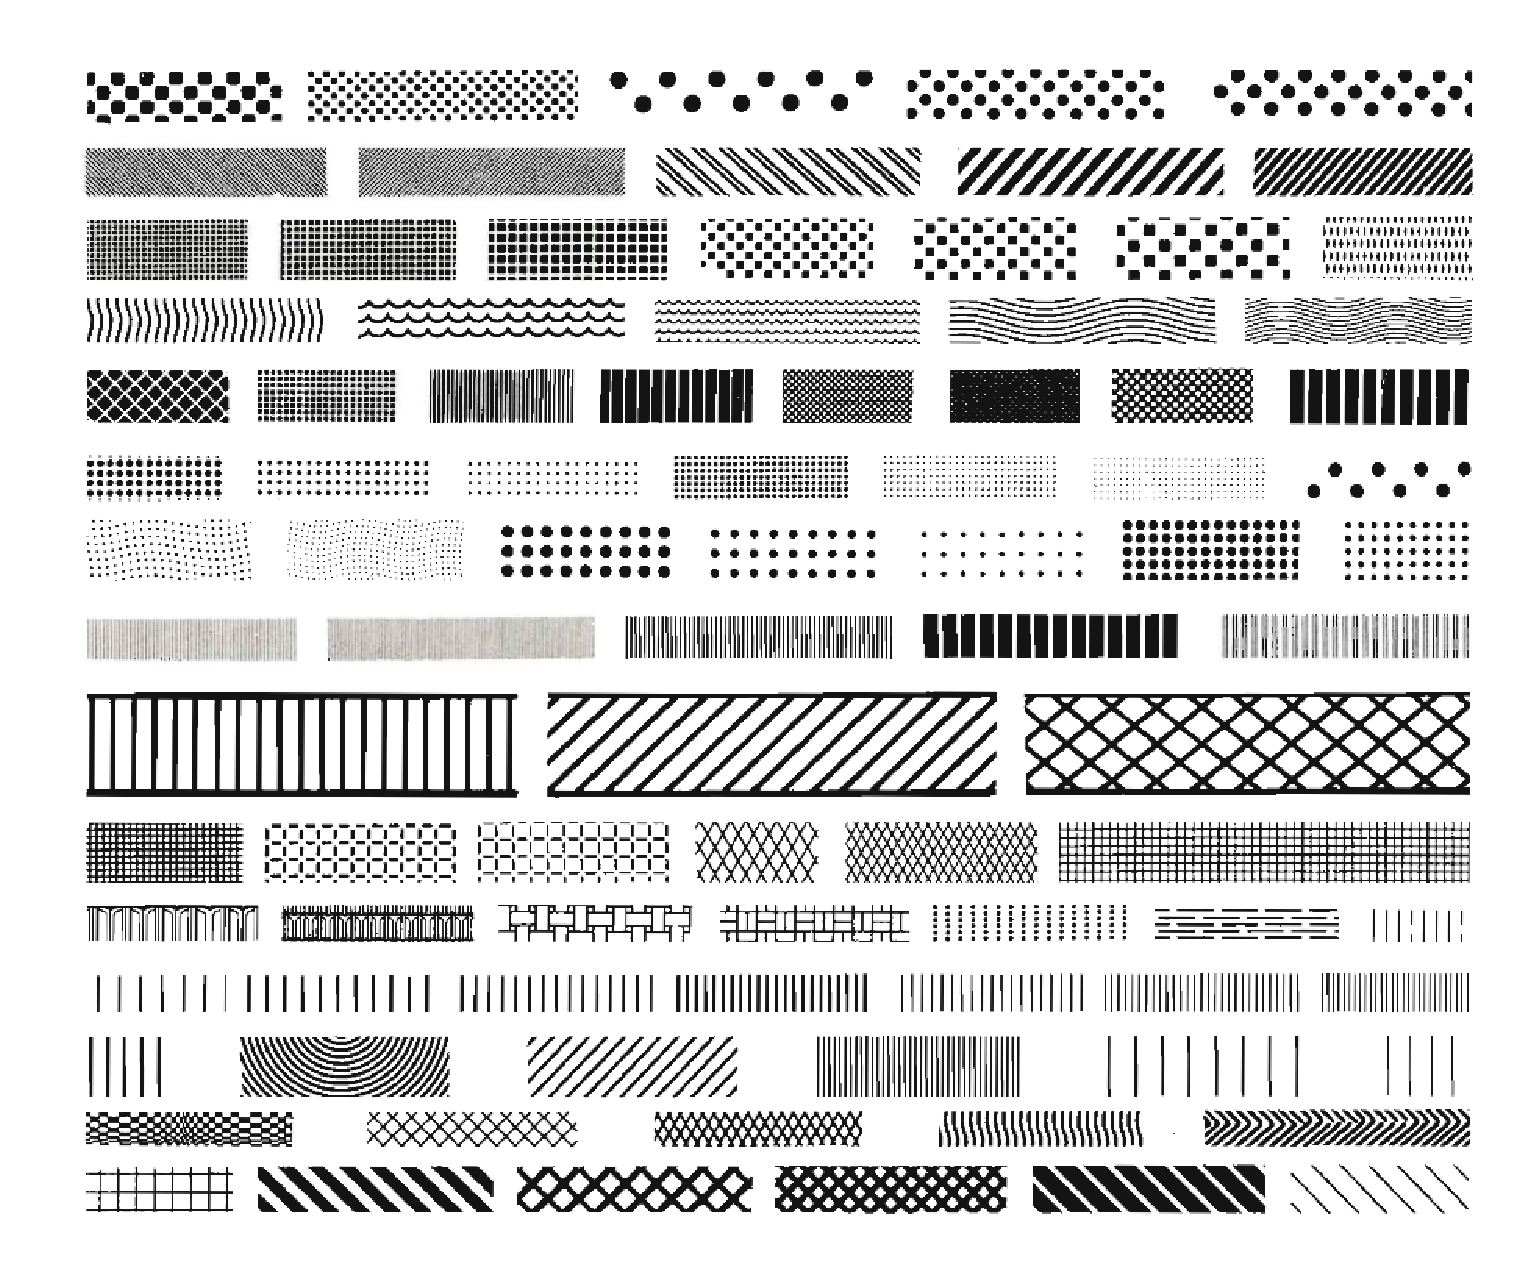
\includegraphics[width=19cm]{./illustrations/annexes/moires.eps}
}
Above, you will find several type of moiré effects. Printing them on a chart make it less clear and less attractive. Considered when computer ploting was created as a modern effect, it has plague ever since chart in the industry. The library shall not encourage this trend.

The grid is also an element that can obfuscate a chart : It compete with the data and is not often necessary.
 It can be useful only when the graph serva as a look-up table, but even then, it shall be lighter than the data and remain in the background. table, but even then, it shall be lighter than the data and remain in the background.
 In those cases, the white grid is a good idea. The white grid is printed by erasing part of the data where a grid should cross it, and not drawing anything else aside of that. Here's an exemple :
%The white grid shall go here
\centerline{
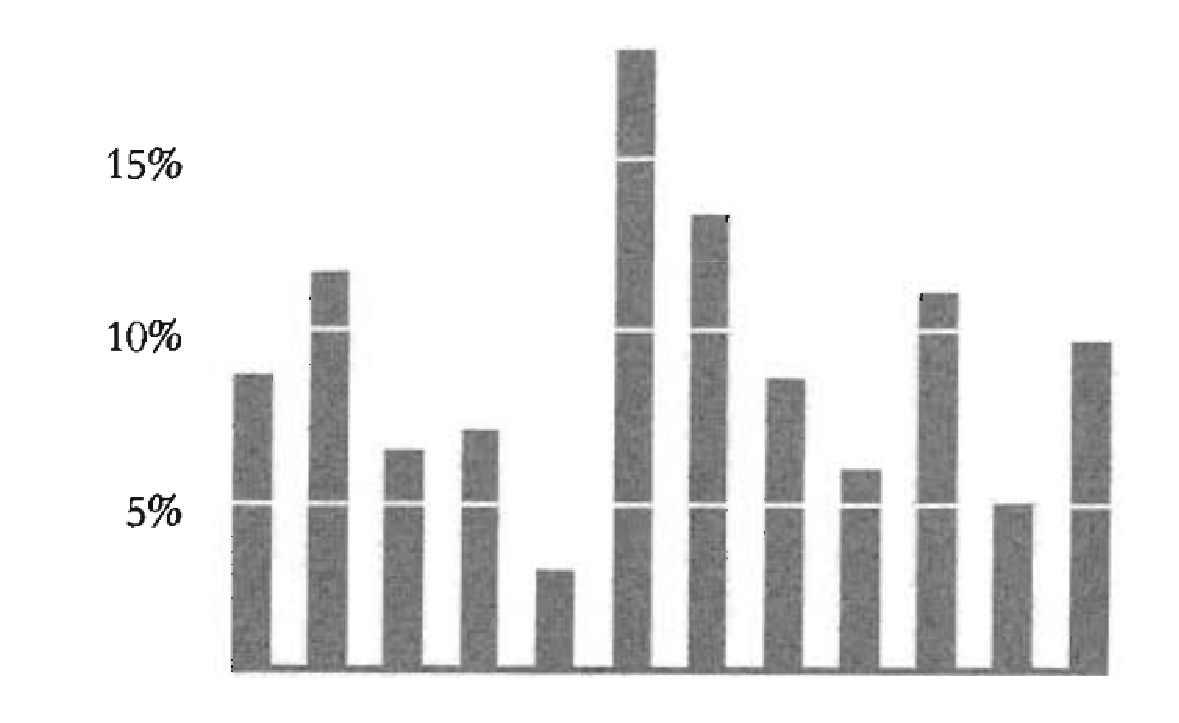
\includegraphics[width=19cm]{./illustrations/annexes/grilleblanche.eps}
}

The axis are also almost never used at their best. By erasing or moving part of it, we can show more data : 

%Image : Chart p.132
\centerline{
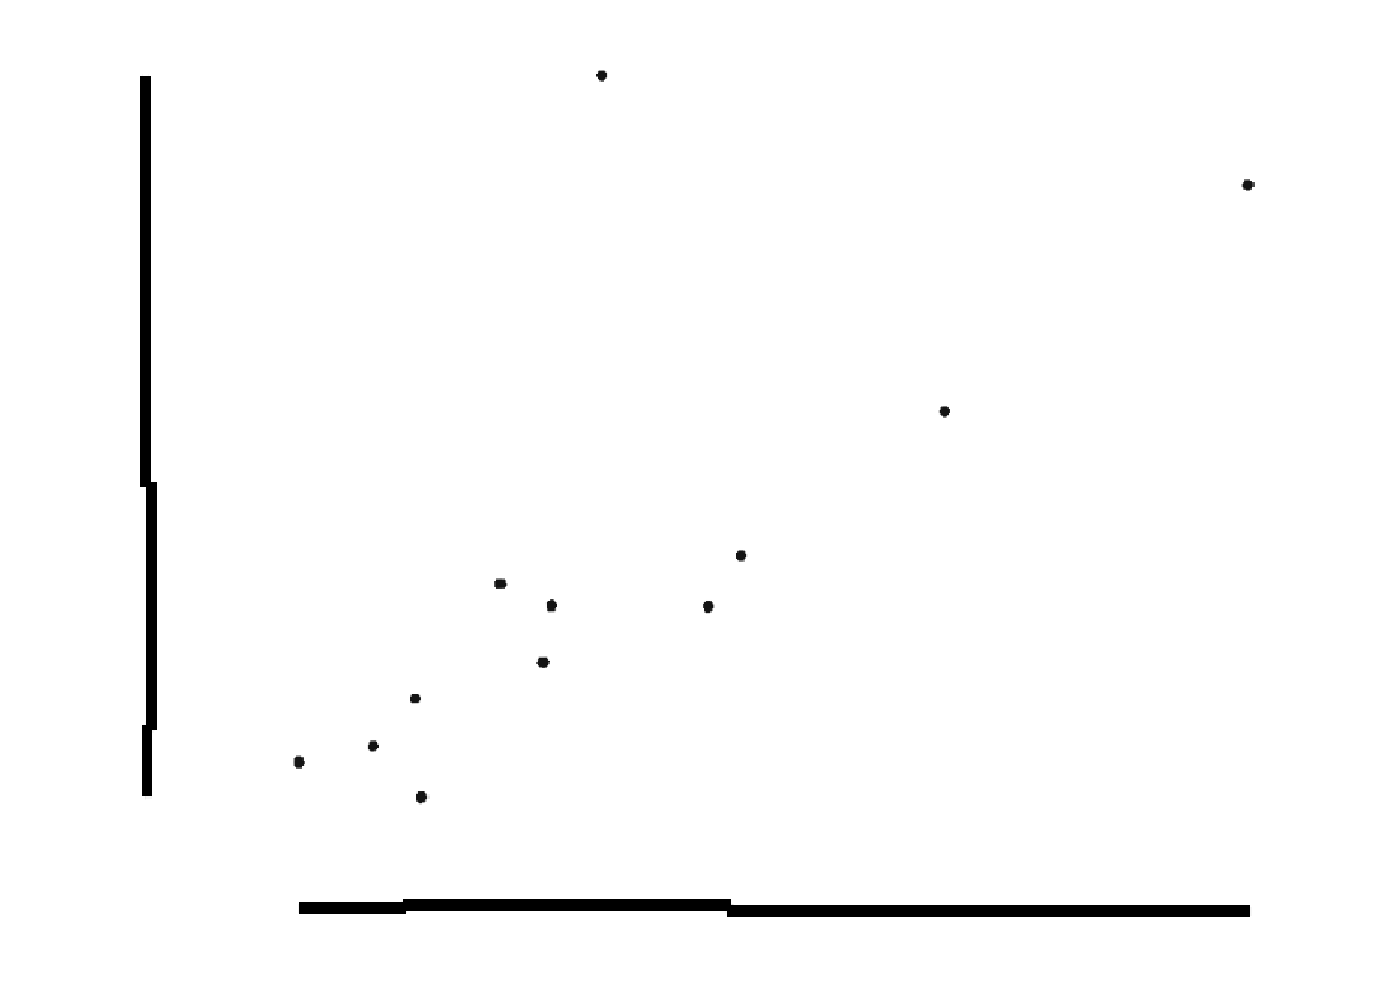
\includegraphics[width=19cm]{./illustrations/annexes/axesmodernes.eps}
}

On this chart, 10 number have been added to the set of data : 
\begin{itemize}
\item the minimum and maximumare shown by begin and ending the axis at their value
\item the shifted part of the axis represent three quartil : lower, upper
\item the erased portion in the shifted part show the median quartil
\end{itemize}
Since these value are showm on the two axis, we have $5*2$ value that have been added.

An axis can also show the marginal distribution of each variables :
%Image : image p.133
\centerline{
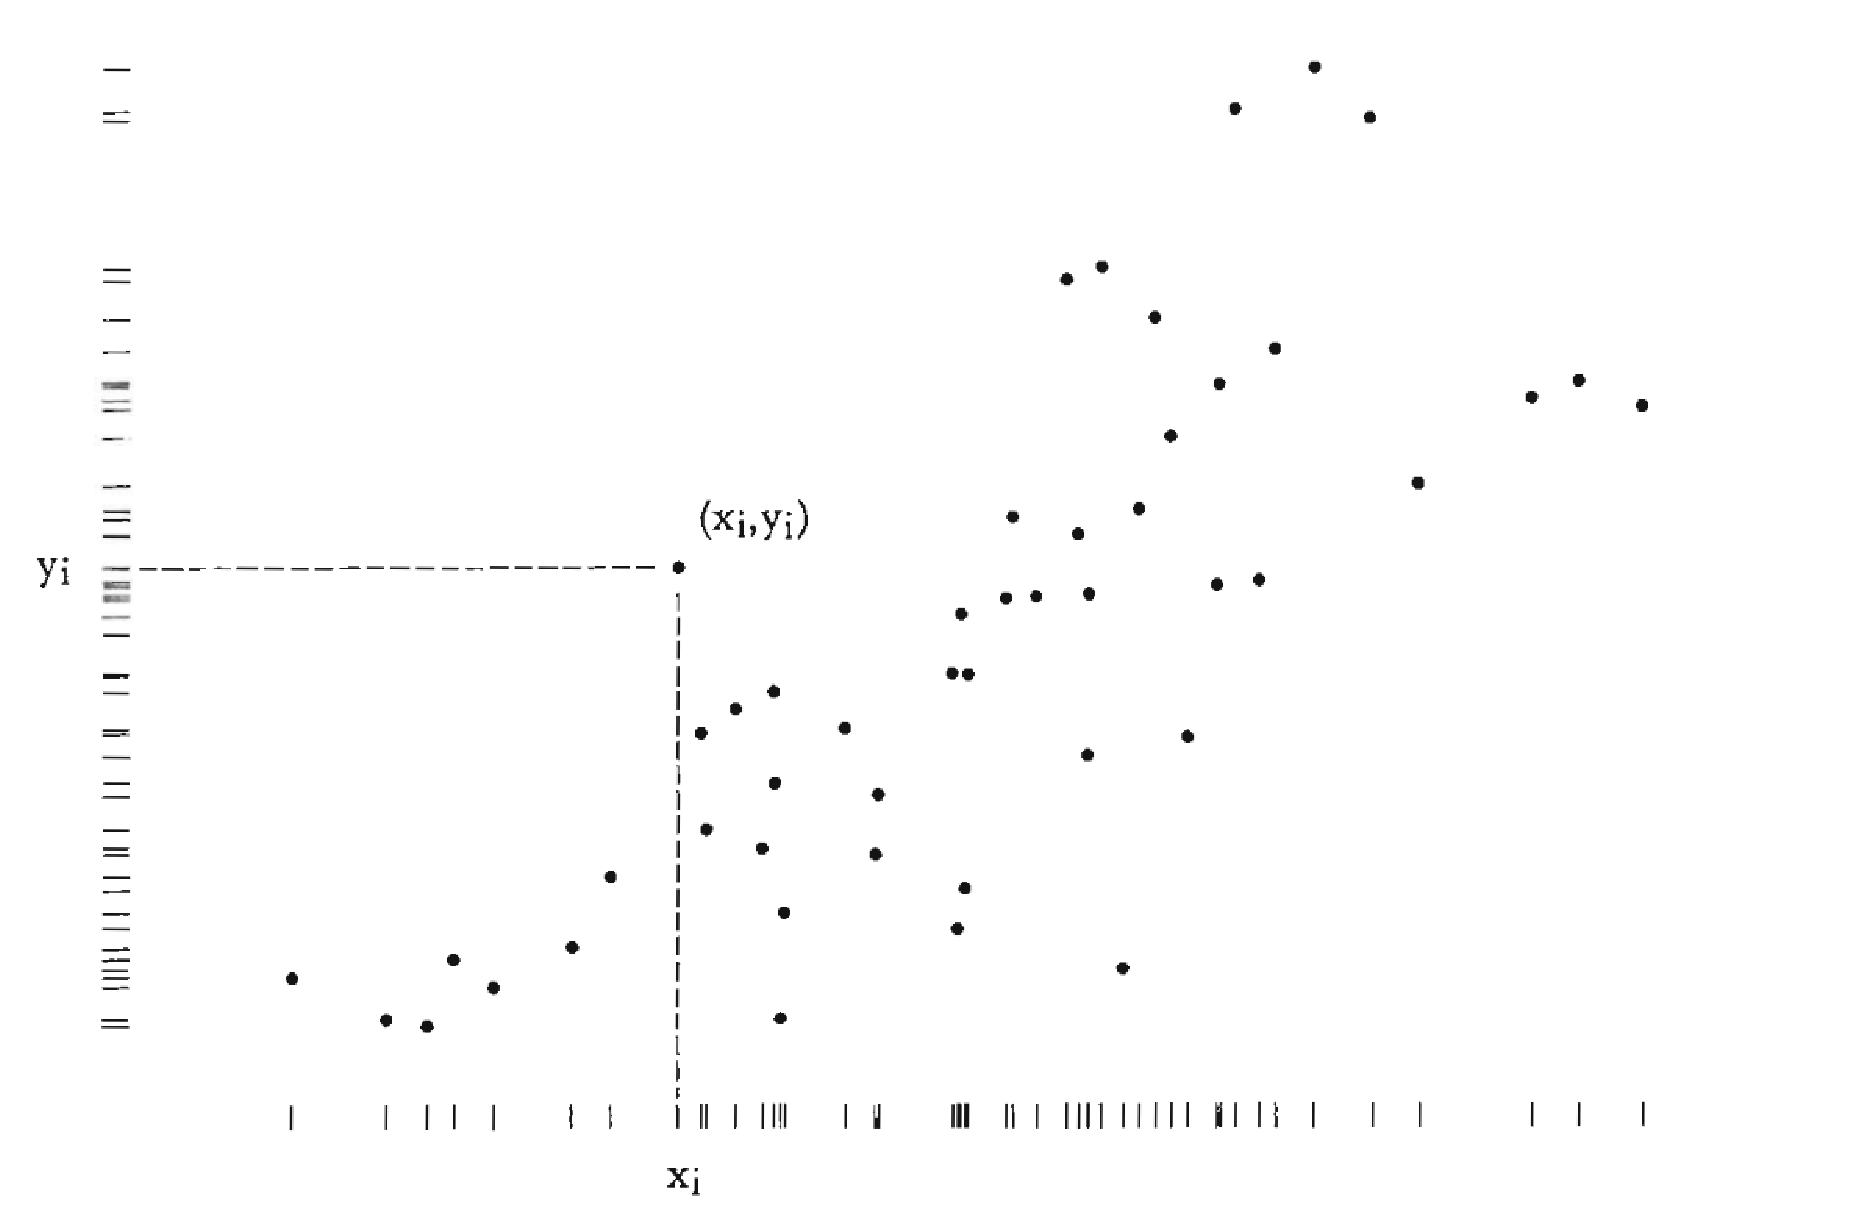
\includegraphics[width=19cm]{./illustrations/annexes/axesdistributions.eps}
}

Ticking is also subjected to improvment : In small set of data, printing actual numbers from the set instead of arbitrary rounded up numbers can also make the axis more efficient.

Effciency in representing data can be found by representing multiple number of information with a single point. A point on a map represent the location, the name of a city and can also represent another variable.
 Push to its limit, this idea can be very interesting : What if the data was represented by its number ? In short to medium sized data set, this idea can sometime be interesting.
 This chart shows, with the economy of one axis, three infotmations : 
\begin{itemize}
\item the number of fivision for each month, June 1917 to October 1918
\item what particular division were in France in each month
\item the duration of each division's presence in France
\end{itemize}
%Image p.141
\centerline{
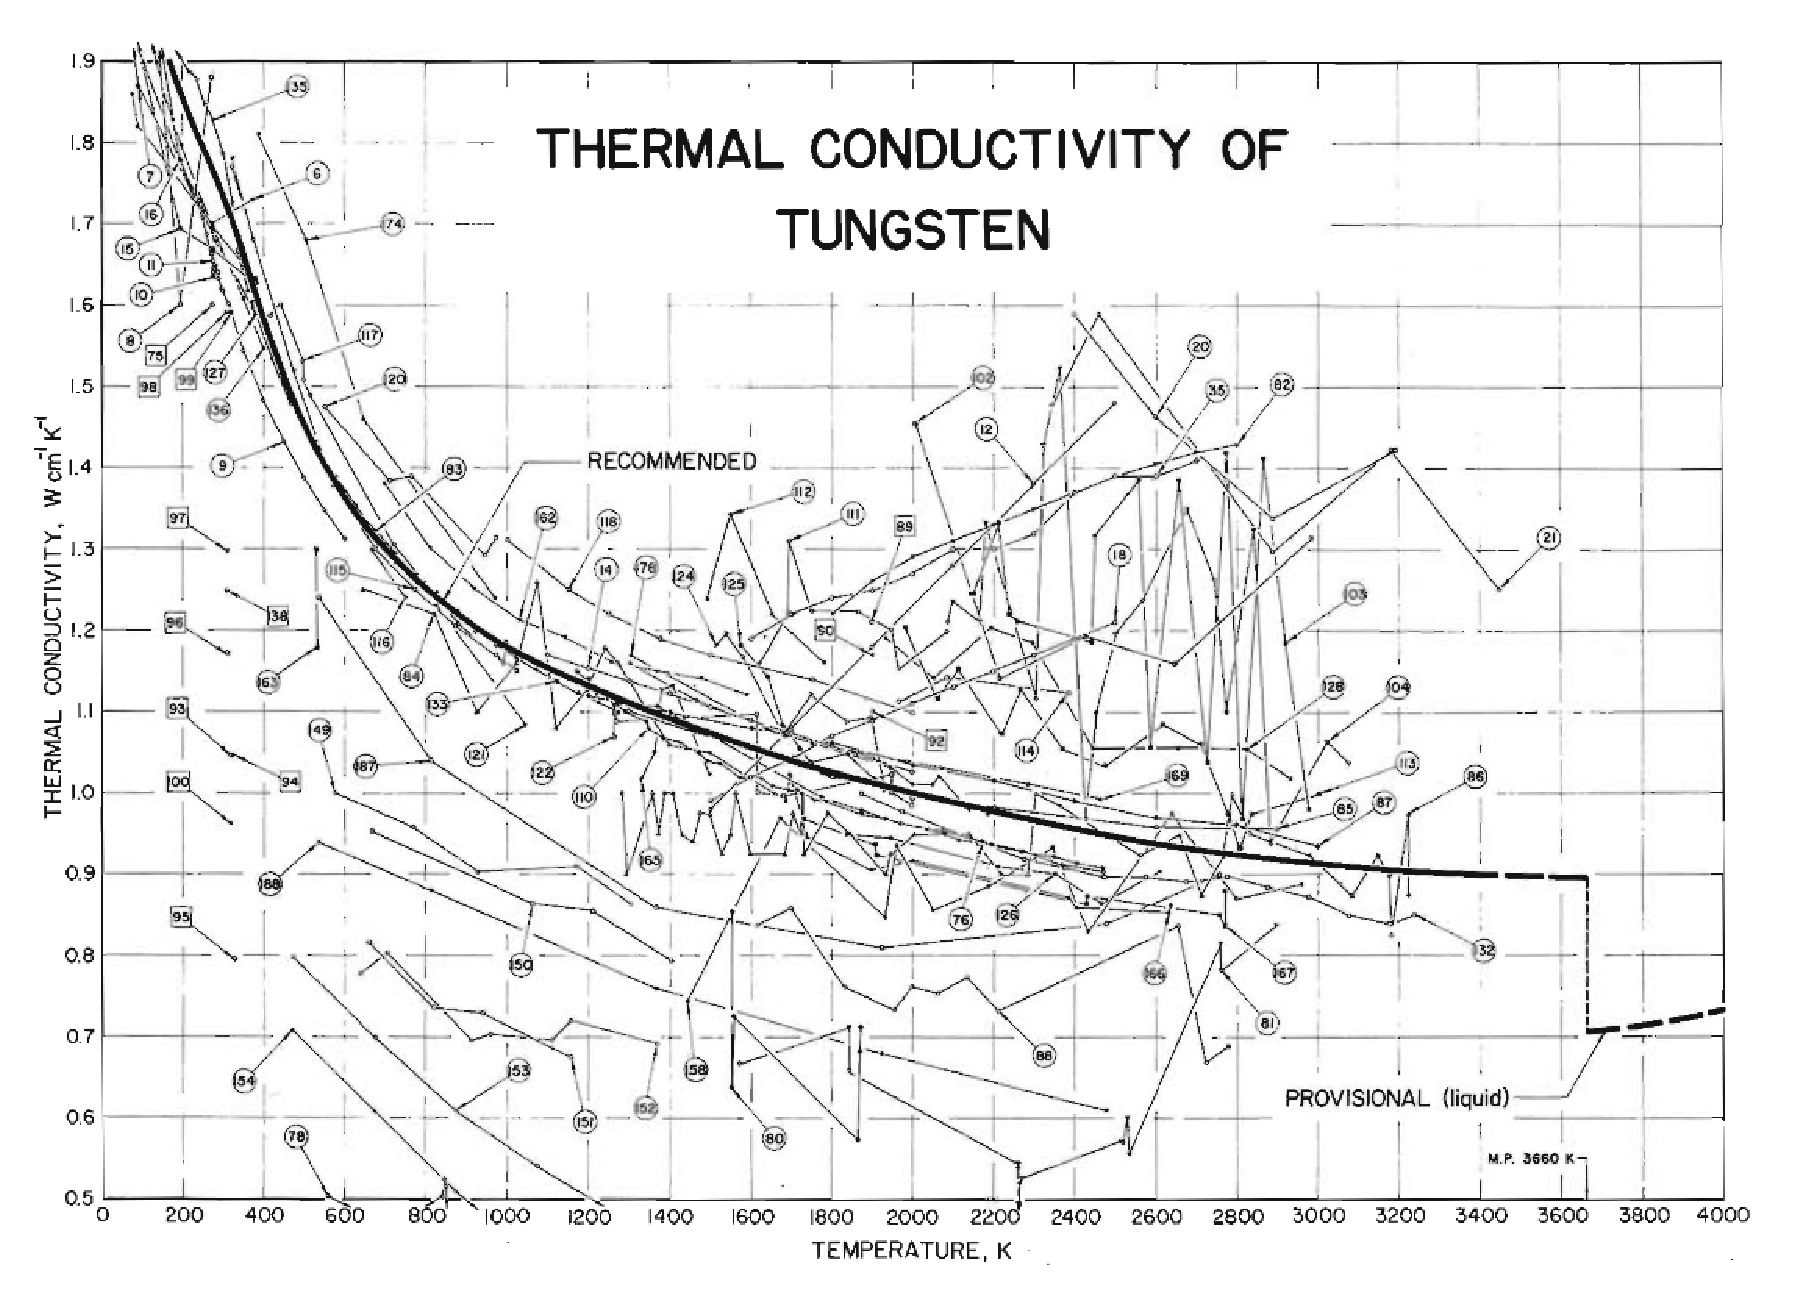
\includegraphics[width=19cm]{./illustrations/annexes/relationel_tungsten.eps}
}
The name given to a data serie can also be interesting if it is chosen wisely.
 If there are a hundread series in a plot, that they are named according to this model : ``61c'' stands for \emph{The third study made in 1961}, and that this name is shown on the plot, it can add a lot of information for the focused viewer.

To judge if a graph is intuitive, the following question should be asked : \emph{Does the viewer see the data or interprate the graphic ? Is my diagram telling a story when glanced at it ? When seen up close, are my data point all making sense ?}
 Color is not often an intuitive medium, for it is not immediately translatable by the viewer in data without jumping to the legend and see what it means. Shade of greys are more efficient. A graphic made of several small graphics can be a very efficient way of showing a lot of data, and compare several states of an object.

Finally, Line weight and lettering should be proportional to the importance of what they represent. Not all of the element should thick, nor should all they be thin. A balance shall be found. A rectangle graphic is also always better.
\section{Conclusion}
%Conclusion here written 

The place of graphic in edition have to be rethink. For small sets of data, wordly graphic or table are preferable, since graphic does not improve much their readability. Graphic should be used for a big sets of data. and they should integrated to text. 
\begin{quote}
Data graphics are paragraphs about data and should be treated as such.
\end{quote}
